\documentclass[]{article}
\newcommand{\FileDepth}{../../..}
\usepackage[letterpaper, landscape, margin=0.5cm]{geometry}
\usepackage[T1]{fontenc}
\usepackage{textcomp}%Not strictly necessary, but gives \textmu command for "micro."
\usepackage{fancyhdr}
\usepackage{amsmath}
\usepackage{amssymb}
\usepackage{graphicx}
\usepackage{xcolor}
\usepackage{tikz}
\usetikzlibrary{calc}
\usepackage[shortlabels]{enumitem}
\usepackage{multicol}
\usepackage{vwcol}
\usepackage{hyperref}
\usepackage{wrapfig}
%opening
\newcommand{\SecType}{L}
\newcommand{\Week}{3}
\title{PH 21X Lecture \Week}
\author{Benjamin Bauml}
\date{Term 2024}

\newcommand{\Purpose}{4}
\newcommand{\DefOnly}{0}

% Version 2024-06-14
% Changes
% 2024-02-21 Added xstring package to enable smooth implementation of new \ModePage command.
% 2024-04-27 Set up to split activities and formatting aspects into separate files. Removed dependence on xcomment. Added an automatic counter to number the activities in a problem set.
% 2024-05-19 Revised old format for \TeachingTips command, which did not support \DefOnly.
% 2024-06-14 Added Repurpose environment to allow mixing of different purpose levels in the same document.
\usepackage{tcolorbox}
\usepackage{xstring}
% You will want the following four lines in your document (the last two uncommented):
% For Assignment, leave Purpose as 1. For Worksheet, set to 2. For Student Solution, set to 3. For Teacher Solution, set to 4.
% If you want keep the pieces from being called manually, set DefOnly to 0.
%\newcommand{\Purpose}{4}
%\newcommand{\DefOnly}{1}
\newcommand{\Exclusion}{0}
\newcommand{\PageTurn}{0}
\newcommand{\GrayProb}{0}
\newcommand{\Tipsy}{0}

% Assignment
\if\Purpose1
\renewcommand{\Exclusion}{1}
\fi
% Worksheet
\if\Purpose2
\renewcommand{\Exclusion}{1}
\renewcommand{\PageTurn}{1}
\fi
% Student Solution
\if\Purpose3
\renewcommand{\PageTurn}{1}
\renewcommand{\GrayProb}{1}
\fi
% Teaching Copy
\if\Purpose4
\renewcommand{\PageTurn}{1}
\renewcommand{\GrayProb}{1}
\renewcommand{\Tipsy}{1}
\fi

\newenvironment{Repurpose}[1]{
\renewcommand{\Purpose}{#1}
\renewcommand{\Exclusion}{0}
\renewcommand{\PageTurn}{0}
\renewcommand{\GrayProb}{0}
\renewcommand{\Tipsy}{0}
% Assignment
\if\Purpose1
\renewcommand{\Exclusion}{1}
\fi
% Worksheet
\if\Purpose2
\renewcommand{\Exclusion}{1}
\renewcommand{\PageTurn}{1}
\fi
% Student Solution
\if\Purpose3
\renewcommand{\PageTurn}{1}
\renewcommand{\GrayProb}{1}
\fi
% Teaching Copy
\if\Purpose4
\renewcommand{\PageTurn}{1}
\renewcommand{\GrayProb}{1}
\renewcommand{\Tipsy}{1}
\fi
}{}

\def \NewQ {0}
\def \PForce {0}
\newcommand{\MaybePage}[1]{
	\def \PForce {#1}
	\if\PForce1
	\newpage
	\else
	\if\NewQ0
	\gdef \NewQ {\PageTurn}
	\else
	\newpage
	\fi
	\fi
}

\newcommand{\ModePage}[1]{
	\IfSubStr{#1}{\Purpose}{\newpage}{}
}

\newcounter{ActNumber}
\setcounter{ActNumber}{0}

\newcommand{\Problem}[4][0]{%The first argument is optional, and if it is set to 1, the \newpage will be forced. The second argument is the name of the activity, the third is the command the activity is stored as, and the fourth is the actual problem statement.
\newcommand{#3}{
\MaybePage{#1}
\addtocounter{ActNumber}{1}
\section*{\SecType\Week-\theActNumber: #2}
\if\GrayProb1
\begin{tcolorbox}[colback=lightgray,colframe=lightgray,sharp corners,boxsep=1pt,left=0pt,right=0pt,top=0pt,bottom=0pt,after skip=2pt]
\else
\begin{tcolorbox}[colback=white,colframe=white,sharp corners,boxsep=1pt,left=0pt,right=0pt,top=0pt,bottom=0pt,after skip=2pt]
\fi
#4
\end{tcolorbox}\noindent
}
\if\DefOnly0
\else
#3
\fi
}
	
\newcommand{\ProblemSub}[3][0]{%The first argument is optional, and if a string of numbers is entered into it, it will force a \newpage in any \Purpose that shows up in the string. For example, "13" would lead to the newpage being forced in modes 1 and 3. The second is the command the activity is stored as, and the third is the actual problem statement.
\newcommand{#2}{
\ModePage{#1}
\if\GrayProb1
\begin{tcolorbox}[colback=lightgray,colframe=lightgray,sharp corners,boxsep=1pt,left=0pt,right=0pt,top=0pt,bottom=0pt,after skip=2pt]
\else
\begin{tcolorbox}[colback=white,colframe=white,sharp corners,boxsep=1pt,left=0pt,right=0pt,top=0pt,bottom=0pt,after skip=2pt]
\fi
#3
\end{tcolorbox}\noindent
}
\if\DefOnly0
\else
#2
\fi
}
		
\newcommand{\Solution}[2]{%The first argument is the command the solution is stored as, and the second is the actual solution.
\newcommand{#1}{
\if\Exclusion0
#2
\fi
}
\if\DefOnly0
\else
#1
\fi
}
		
\newcommand{\ProblemFig}[2]{%The first argument is the command the figure is stored as, and the second is the actual figure.
\newcommand{#1}{
\begin{figure}[h]
#2
\end{figure}
}
\if\DefOnly0
\else
#1
\fi
}

\newcommand{\TeachingTips}[2]{%The first argument is the command the tip is stored as, and the second is the actual tip.
\newcommand{#1}{
\if\Tipsy1
\begin{tcolorbox}[colback=lightgray,colframe=black]
#2
\end{tcolorbox}
\fi
}
\if\DefOnly0
\else
#1
\fi
}
\usepackage[absolute]{textpos}
% This package relies on Assignment Format 2024-06-14 or later to work. It is recommended that the Purpose and DefOnly commands be given as such:
%\newcommand{\Purpose}{4}
%\newcommand{\DefOnly}{0}
% Activities need to be entered outside of the TeacherMargin and PresentSpace environments, otherwise they will be defined only locally. They can even go in the preamble.
\newenvironment{TeacherMargin}{\begin{textblock*}{10.8cm}(0.5cm,0.5cm)
\small}{\end{textblock*}
\hspace{0.1cm}}
\newenvironment{PresentSpace}{\begin{textblock*}{0.3cm}(26.85cm,9.35cm)
--
\end{textblock*}
\begin{textblock*}{0.3cm}(26.85cm,18.7cm)
--
\end{textblock*}
\begin{textblock*}{0.3cm}(26.85cm,12.24cm)
	--
\end{textblock*}
\begin{textblock*}{15.6cm}(11.8cm,0.5cm)
\begin{Repurpose}{1}
\Large}{\end{Repurpose}
\end{textblock*}
\hspace{0.1cm}}

%\newcommand{\FBDaxes}[3]{
	\begin{scope}[shift={(#1)},rotate=#2]
		% x-axis
		\draw[thick,->] (-2,0) -- (2,0);
		\node[anchor=west] at (2,0) {$x$};
		% y-axis
		\draw[thick,->] (0,-2) -- (0,2);
		\node[anchor=west] at (0,2) {$y$};
		\coordinate (#3) at (0,0);
	\end{scope}
}
\newcommand{\FBDvectorMA}[4]{
	\begin{scope}[shift={(#1)}]
		\coordinate (#4tip) at ({#2*cos(#3)},{#2*sin(#3)});
		\draw[ultra thick,blue,->] (#1) -- (#4tip);
	\end{scope}
}
\newcommand{\FBDvectorXY}[3]{
	\begin{scope}[shift={(#1)}]
		\coordinate (#3tip) at (#2);
		\draw[ultra thick,blue,->] (0,0) -- (#3tip);
	\end{scope}
}
\newcommand{\FBDdot}[1]{
	\filldraw[black] (#1) circle (3pt);
}
%\newcommand{\MVec}[3][0]{%Creates a momentum vector of length #3 centered at #2 and rotated #1 degrees counterclockwise.
	\begin{scope}[rotate=#1,shift={(#2)}]
		\draw[->,thick] ({-#3/2},0) -- ({#3/2},0);
	\end{scope}
}
\newcommand{\MDot}[1]{%Creates a dot at #1 to represent a zero vector.
	\filldraw (#1) circle (1pt);
}
\newcommand{\MVDRows}[2][4.5]{%Creates the rows (initial, delta, final) of a momentum vector diagram. The optional argument determines the width of the table, and defaults to a good length for three columns (two objects and the total system). The non-optional argument gives a coordinate name (not displayed) to the diagram.
	\begin{scope}
		%\draw[thick] (0,5.5) -- (0,0);
		\draw[thick] (-1,4.5) -- (#1,4.5);
		\node at (-0.5,3.75) {$\vec{p}_{i}$};
		\draw[thick] (-1,3) -- (#1,3);
		\node at (-0.5,2.25) {$\Delta\vec{p}$};
		\draw[thick] (-1,1.5) -- (#1,1.5);
		\node at (-0.5,0.75) {$\vec{p}_{f}$};
		\coordinate (#2) at (0,5);
	\end{scope}
}
\newcommand{\MVDCol}[4][0.75]{%Creates a column for an object in a momentum vector diagram. The first (non-optional) argument is the coordinate name (not displayed) of the column, while the second is the displayed column header. The first argument also names the three entries down the column. The third argument anchors the column, so it should either be the coordinate name of the MVD (for the first column) or the coordinate name of the previous column. The optional argument indicates how far the center of the column should be from the previous column's edge, and defaults to 0.75
	\begin{scope}[shift={(#4)}]
		\node at (#1,0) {#3};
		%\draw[thick] ({#1*2},0.5) -- ({#1*2},-5);
		\draw[thick] (0,0.5) -- (0,-5);
		\coordinate (#2init) at (#1,-1.25);
		\coordinate (#2delt) at (#1,-2.75);
		\coordinate (#2fin) at (#1,-4.25);
		\coordinate (#2) at ({#1*2},0);
	\end{scope}
}

%\input{\FileDepth/Activities/Activity_One/Activity_One.tex}
%\input{\FileDepth/Activities/Activity_Two/Activity_Two.tex}

\begin{document}
\begin{TeacherMargin}

\end{TeacherMargin}
\begin{PresentSpace}
\begin{center}
	\huge Lecture 3: Acceleration
\end{center}
\vspace{1cm}
\underline{Warm-Up Activity} \\
For an object moving in one dimension (in a straight line), what does it mean if the acceleration and the velocity are in opposite directions? The object is\dots
\begin{enumerate}[(A)]
	\item Slowing Down
	\item Speeding Up
	\item Staying Still
	\item Not Enough Information
\end{enumerate}
\end{PresentSpace}
\newpage
\begin{TeacherMargin}
The members of the instructional team who are performing assessment have limits on their time. We cannot guarantee that we will be able to take time to assess late work, or that we will be able to give feedback on all parts of an assignment. We may elect to assess a subset of the problems in a given assignment.
\end{TeacherMargin}
\begin{PresentSpace}
\section*{Homework}
\begin{itemize}
	\item Physics homework is not (just) about getting correct answers.
	\item The homework format is designed to help you \textbf{communicate the depth of your physics knowledge and	understanding} and \textbf{learn how to break down a problem}.
	\item Make sure you submit an organized and clear submission!
\end{itemize}
\vspace{2.5cm}
\section*{Late Work}
\begin{itemize}
	\item If you need an extension, ask first.
	\item If you miss a deadline, you should still turn it in when you are ready.
	\item Assignments turned in after the deadline without an approved extension may not receive feedback.
	\item If you need more feedback on a problem (even a problem that missed the deadline), reach out to us in the Wormhole and in office hours.
\end{itemize}
\end{PresentSpace}
\newpage
\begin{TeacherMargin}

\end{TeacherMargin}
\begin{PresentSpace}
\textbf{A Model for Motion}
\begin{multicols}{2}
	Quantities
	\begin{itemize}
		\item Position: $\vec{r}$
		\item Velocity: $\vec{v}=\frac{d\vec{r}}{dt}$
		\item Acceleration: $\vec{a}=\frac{d\vec{v}}{dt}$
	\end{itemize}
	\vspace{1cm}
	Assumptions
	\begin{itemize}
		\item Use the Particle Model
	\end{itemize}
\end{multicols}
Motion Diagram
\begin{figure}[h]
	\centering
	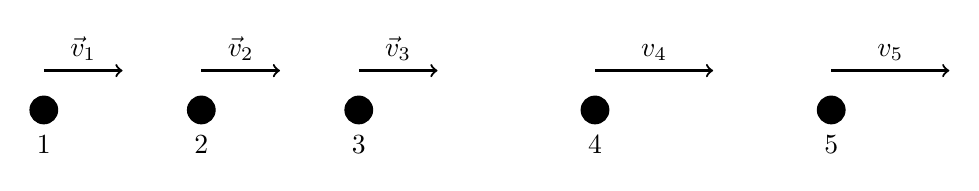
\begin{tikzpicture}
		\foreach \x in {1,2,3}
			\filldraw (2*\x,0) circle (5pt);
		\foreach \x in {1,2,3}
			\node[anchor=north] at (2*\x,-0.2) {\x};
		\foreach \x in {1,2,3}
			\draw[thick,->] (2*\x,0.5) -- (2*\x+1,0.5);
		\foreach \x in {1,2,3}
			\node[anchor=south] at (2*\x+0.5,0.5) {$\vec{v}_{\x}$};
		\begin{scope}[shift={(-3,0)}]
			\foreach \x in {4,5}
				\filldraw (3*\x,0) circle (5pt);
			\foreach \x in {4,5}
				\node[anchor=north] at (3*\x,-0.2) {\x};
			\foreach \x in {4,5}
				\draw[thick,->] (3*\x,0.5) -- (3*\x+1.5,0.5);
			\foreach \x in {4,5}
				\node[anchor=south] at (3*\x+0.75,0.5) {$v_{\x}$};
		\end{scope}
	\end{tikzpicture}
\end{figure}
\end{PresentSpace}
\newpage
\begin{TeacherMargin}
\section*{L3-1: Direction of Velocity and Acceleration}
\begin{center}
	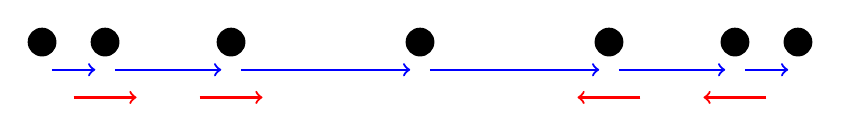
\begin{tikzpicture}
		\foreach \x in {0,1,2,3,4}
			\filldraw (2.4*\x,0) node[shift={(0,-10pt)}] (dot\x) {} circle (5pt);
		\filldraw (0.8,0) node[shift={(0,-10pt)}] (dottwo) {} circle (5pt);
		\filldraw (8.8,0) node[shift={(0,-10pt)}] (dotsix) {} circle (5pt);
		\draw[thick,blue,->] (dot0) -- (dottwo);
		\draw[thick,blue,->] (dottwo) -- (dot1);
		\draw[thick,blue,->] (dot1) -- (dot2);
		\draw[thick,blue,->] (dot2) -- (dot3);
		\draw[thick,blue,->] (dot3) -- (dotsix);
		\draw[thick,blue,->] (dotsix) -- (dot4);
		\begin{scope}[shift=(dottwo)]
			\draw[thick,red,->] (-0.4,-10pt) -- (0.4,-10pt);
		\end{scope}
		\begin{scope}[shift=(dot1)]
			\draw[thick,red,->] (-0.4,-10pt) -- (0.4,-10pt);
		\end{scope}
		\begin{scope}[shift=(dot3)]
			\draw[thick,red,->] (0.4,-10pt) -- (-0.4,-10pt);
		\end{scope}
		\begin{scope}[shift=(dotsix)]
			\draw[thick,red,->] (0.4,-10pt) -- (-0.4,-10pt);
		\end{scope}
	\end{tikzpicture}
\end{center}
We can approximate the velocity vectors using the definition of average velocity:
\[
\vec{v}_{avg} = \frac{\Delta\vec{r}}{\Delta t}.
\]
Using a forward approximation, we will take $\Delta\vec{r}$ to be the displacement from one dot to the next, and estimate the velocity of the first dot to be the calculated average velocity.
\begin{center}
	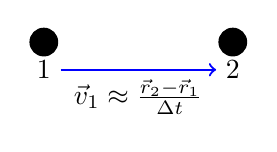
\begin{tikzpicture}
		\foreach \x in {1,2}
			\filldraw (2.4*\x,0) node[shift={(0,-10pt)}] (dot\x) {\x} circle (5pt);
		\draw[thick,blue,->] (dot1) -- (dot2);
		\node[anchor=north] at (3.6,-10pt) {$\vec{v}_{1} \approx \frac{\vec{r}_{2}-\vec{r}_{1}}{\Delta t}$};
	\end{tikzpicture}
\end{center}
We can approximate the acceleration vectors using the definition of average acceleration:
\[
\vec{a}_{avg} = \frac{\Delta\vec{v}}{\Delta t}.
\]
This will be a rougher approximation, as we are using approximate velocities instead of instantanous velocities. It appears rather natural to determine $\Delta\vec{v}$ at a dot by taking the vector pointing to it from the previous dot and subtracting it from the vector pointing from it to the next dot---which is technically a backward approximation.
\begin{center}
	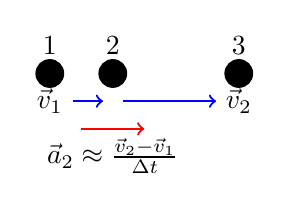
\begin{tikzpicture}
		\node at (2.4,10pt) {1};
		\node at (3.2,10pt) {2};
		\node at (4.8,10pt) {3};
		\foreach \x in {1,2}
			\filldraw (2.4*\x,0) node[shift={(0,-10pt)}] (dot\x) {$\vec{v}_{\x}$} circle (5pt);
		\filldraw (3.2,0) node[shift={(0,-10pt)}] (dottwo) {} circle (5pt);
		\draw[thick,blue,->] (dot1) -- (dottwo);
		\draw[thick,blue,->] (dottwo) -- (dot2);
		\begin{scope}[shift=(dottwo)]
			\draw[thick,red,->] (-0.4,-10pt) -- (0.4,-10pt);
		\end{scope}
		\node[anchor=north] at (3.2,-20pt) {$\vec{a}_{2} \approx \frac{\vec{v}_{2}-\vec{v}_{1}}{\Delta t}$};
	\end{tikzpicture}
\end{center}
\begin{enumerate}[(a)]
	\item When acceleration is zero, the velocity does not change. This happens in the middle of the motion diagram.
	\item When acceleration and velocity are in opposite directions, the object slows down (the velocity decreases in magnitude). This happens on the right side of the motion diagram.
	\item When acceleration and velocity are in the same direction, the object speeds up (the velocity increases in magnitude). This happens on the left side of the motion diagram.
\end{enumerate}
%Motion graphs are a little up to interpretation, but the following are one possibility. Recall that $v=\frac{dx}{dt}$ and $a=\frac{dv}{dt}$.
\begin{comment}
	\begin{tikzpicture}
		\begin{scope}
			\draw[thick,<->] (0,3) node[anchor=south] {$x$} -- (0,0) -- (3,0) node[anchor=west] {$t$};
			\draw[thick,domain=0:1.125,variable=\t] plot ({\t},{1.19*\t*\t});
			\draw[thick,domain=1.825:3,variable=\t] plot ({\t},{5.25-1.19*(\t-3)*(\t-3)});
			\draw[thick] (1.125,1.5) -- (1.825,3.6);
			%\draw[thick,domain=0:3,variable=\t] plot ({\t},{3*\t*\t/4-\t*\t*\t/6});
		\end{scope}
		\begin{scope}[shift={(4,0)}]
			\draw[thick,<->] (0,3) node[anchor=south] {$v$} -- (0,0) -- (3,0) node[anchor=west] {$t$};
			\draw[thick,blue] (0,0) -- (1.125,1.125) -- (1.825,1.125) -- (3,0);
			%\draw[thick,blue] (0,0) -- (1.125,1.125) .. controls (1.5,1.45) .. (1.825,1.125) -- (3,0);
			%\draw[thick,domain=0:3,variable=\t] plot ({\t},{\t*(3-\t)/2});
		\end{scope}
		\begin{scope}[shift={(8,0)}]
			\draw[thick,<->] (0,3) node[anchor=south] {$a$} -- (0,0) -- (0,1.5) -- (3,1.5) node[anchor=west] {$t$};
			\draw[thick,red] (0,2.5) -- (1.125,2.5);
			\draw[thick,dashed,red] (1.125,2.5) -- (1.125,1.5);
			\draw[thick,red] (1.125,1.5) -- (1.825,1.5);
			\draw[thick,dashed,red] (1.825,1.5) -- (1.825,0.5);
			\draw[thick,red] (1.825,0.5) -- (3,0.5);
			%\draw[thick,red] (0,2.5) -- (1.125,2.5) -- (1.825,0.5) -- (3,0.5);
		\end{scope}
	\end{tikzpicture}
\end{comment}
\end{TeacherMargin}
\begin{PresentSpace}
\section*{L3-1: Direction of Velocity and Acceleration}
\begin{center}
	
\begin{tikzpicture}
		\foreach \x in {0,1,2,3,4}
			\filldraw (2.4*\x,0) circle (5pt);
		\filldraw (0.8,0) circle (5pt);
		\filldraw (8.8,0) circle (5pt);
	\end{tikzpicture}
\end{center}
\vspace{0.25cm}
\begin{itemize}
	\item The motion diagram above shows a ball moving from left to right.
	\begin{itemize}
		\item Draw velocity and acceleration vectors at each instant.
	\end{itemize}
	\item For an object moving in one dimension (in a straight line), what does it mean if:
	\begin{enumerate}[(a)]
		\item The acceleration is zero?
		\item The acceleration and the velocity are in opposite directions?
		\item The acceleration and the velocity are in the same direction?
	\end{enumerate}
\end{itemize}
\end{PresentSpace}
\newpage
\begin{TeacherMargin}

\end{TeacherMargin}
\begin{PresentSpace}
\vspace{-10pt}
\section*{L3-2: Vax'ildan's Acceleration}
\vspace{-20pt}
\begin{multicols}{2}
\begin{itemize}
	\item Vax'ildan Vessar is initially located at position $x_{i}$, running to the right with initial speed $v_{i}$.
	\item At $t=0$, Vax clicks his \textit{boots of haste}, which provide an acceleration:
	\vspace{-10pt}
	\[
	\vec{a}(t) = a_{0}\left(1-\frac{t}{T}\right)\hat{x}
	\]
	\vspace{-20pt}
	\item Our goals are:
	\begin{itemize}
		\item Find how much time it takes for Vax to return to his initial velocity.
		\item Find Vax's position at this time.
	\end{itemize}
\end{itemize}
\begin{center}
\reflectbox{
\includegraphics[scale=0.15]{Vax-Linda_Lithen}}
\end{center}
\end{multicols}
%\vspace{1.5cm}
\section*{Solving an ARCS Problem}
\begin{center}
	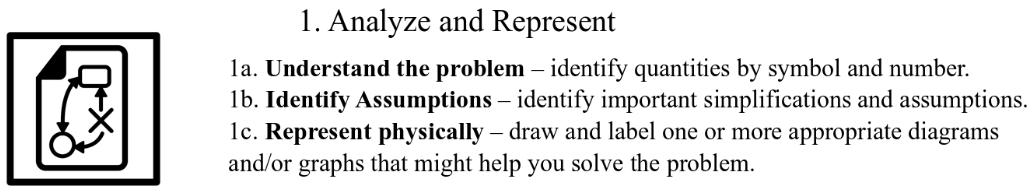
\includegraphics[scale=0.4]{AnalyzeAndRepresent}
	
\includegraphics[scale=0.4]{Calculate}
	
\includegraphics[scale=0.4]{Sensemake}
\end{center}
\begin{comment}
	\item \textbf{A}nalyze \& \textbf{R}epresent
	\begin{center}
		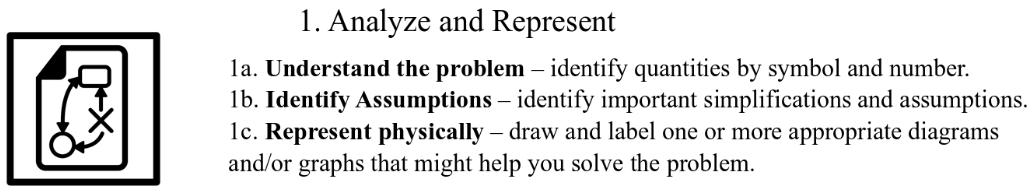
\includegraphics[scale=0.4]{AnalyzeAndRepresent}
	\end{center}
	\item \textbf{C}alculate
	\item \textbf{S}ensemake
\end{comment}
\end{PresentSpace}
\newpage
\begin{TeacherMargin}
We need $1-\frac{t}{T}$ to be unitless, because 1 is unitless, so $t/T$ must also be. Since $t$ is in seconds, it follows that $T$ must also be.

Note that, when we plug in $t = T$, we find that $\vec{a}(T) = 0\hat{x}$, so the acceleration burst stops after $T$ passes, at which point the acceleration changes direction to bring Vax back to his initial velocity. As such, $T$ can be thought of as the duration of the acceleration burst.

Since $\left(1-\frac{t}{T}\right)\hat{x}$ is unitless, the overall units of the right hand side come from $a_{0}$. We need the right hand side to be an acceleration to match the left, so $a_{0}$ has units of m/s$^{2}$.

Note that, when we plug in $t=0$ s, we find that $\vec{a}(0\text{ s})=a_{0}\hat{x}$, so $a_{0}$ is the magnitude of the initial acceleration.

The unit vector $\hat{x}$ carries all of the direction information. It tells us that the acceleration is in the $x$-direction (though left or right depends on the sign).

\noindent\textbf{Understand and Plan}
\vspace{-10pt}
\begin{multicols}{2}
	\noindent\textbf{Knowns}
	\begin{itemize}
		\item Initial Position: $x_{i} = 0$ m (simplifying assumption)
		\item Initial Velocity: $v_{i} = 2$ m/s (a reasonable speed to estimate for a half-elf)
		\item $T = 6$ s (rounds in \textit{Dungeons \& Dragons} last six seconds)
		\item $a_{0} = 0.5$ m/s$^{2}$ (significantly less than free-fall acceleration)
	\end{itemize}
	\noindent\textbf{Unknowns}
	\begin{itemize}
		\item When Vax returns to his initial velocity: $t_{f}$
		\item Vax's final position: $x_{f}$
		\item Equations of motion for velocity and position: $\vec{v}(t)$ and $\vec{x}(t)$
	\end{itemize}
\end{multicols}
\vspace{-10pt}
\noindent\textbf{Identify Assumptions}
\begin{itemize}
	\item Particle Model
	\begin{itemize}
		\item We do not wish to handle the complexities of how Vax's arms, legs, and wings move as he runs, so we will treat him as a point mass.
	\end{itemize}
	\item 1-D Motion
	\begin{itemize}
		\item We will assume Vax is travelling over relatively level ground so we do not have to consider Vax's vertical motion.
	\end{itemize}
	\item Vax is not obstructed in his movement.
	\begin{itemize}
		\item If Vax were to bump into something, that brief interaction would alter his motion in additional ways that the acceleration of the boots does not account for.
	\end{itemize}
\end{itemize}
\noindent\textbf{Represent Physically}
\vspace{-10pt}
\begin{center}
	\begin{tikzpicture}
		\draw[thick,->] (0,-2.2) -- (0,2.2) node[anchor=south] {$a(t)$};
		\draw[thick,->] (0,0) -- (4.2,0) node[anchor=west] {$t$};
		\draw[thick] (2,4pt) -- (2,-4pt) node[anchor=north] {$T$};
		\draw[thick] (4,4pt) -- (4,-4pt) node[anchor=north] {$2T$};
		\draw[thick] (-4pt,2) node[anchor=east] {$a_{0}$} -- (0,2);
		\draw[thick,blue] (0,2) -- (4,-2);
	\end{tikzpicture}
\end{center}
\end{TeacherMargin}
\begin{PresentSpace}
\vspace{-10pt}
\section*{L3-2: Vax'ildan's Acceleration -- Analyze \& Represent}
\vspace{-20pt}
\begin{multicols}{2}
\begin{itemize}
	\item Vax'ildan Vessar is initially located at position $x_{i}$, running to the right with initial speed $v_{i}$.
	\item At $t=0$, Vax clicks his \textit{boots of haste}, which provide an acceleration:
	\[
	\vec{a}(t) = a_{0}\left(1-\frac{t}{T}\right)\hat{x}
	\]
	\vspace{40pt}
	\item With your group:
	\begin{itemize}
		\item What are the units of $T$ and $a_{0}$? What do they represent physically?
		\item What does $\hat{x}$ mean?
		\item \textbf{Understand and Plan:} Identify quantities by symbol and number.
		\item \textbf{Identify Assumptions}
		\item \textbf{Represent Physically}
		\begin{itemize}
			\item What does $\vec{a}(t)$ look like?
		\end{itemize}
	\end{itemize}
\end{itemize}
\end{multicols}
\end{PresentSpace}
\newpage
\begin{TeacherMargin}

\end{TeacherMargin}
\begin{PresentSpace}
\section*{Main Ideas}
\begin{itemize}
	\item If we know the acceleration of an object as a function of time, we can determine the velocity as a function of time.
	\item If we know the velocity as a function of time, we can determine the position as a function of time.
\end{itemize}
\end{PresentSpace}
\end{document}